\documentclass[11pt,a4paper]{article}

\usepackage[margin=2.0cm]{geometry}
\usepackage{amsmath,amssymb,amsfonts}
\usepackage[T1]{fontenc}
\usepackage{lmodern}
\usepackage{microtype}
\usepackage{enumitem}
\usepackage{booktabs}
\usepackage{tabularx}
\usepackage{multirow}
\usepackage{xcolor}
\usepackage[hidelinks,colorlinks=true,
            urlcolor=blue!50!black,
            linkcolor=blue!50!black,
            citecolor=blue!50!black]{hyperref}
\usepackage{listings}
\usepackage{tikz}
\usepackage{pgfplots}
\pgfplotsset{compat=1.18}
\usetikzlibrary{positioning,arrows.meta,shapes.geometric,fit,calc,
                decorations.pathreplacing,trees,backgrounds}

\definecolor{matclr}{RGB}{40,103,160}
\definecolor{unitclr}{RGB}{180,70,40}
\definecolor{rawclr}{RGB}{50,140,80}
\definecolor{prodclr}{RGB}{160,60,140}
\definecolor{kept}{RGB}{40,140,80}
\definecolor{cut}{RGB}{170,60,60}
\definecolor{accent}{RGB}{200,120,30}
\definecolor{hsikan}{RGB}{40,103,160}
\definecolor{sgcn}{RGB}{160,60,140}
\definecolor{sgt}{RGB}{200,120,30}
\definecolor{dad}{RGB}{120,120,120}
\definecolor{win}{RGB}{40,140,80}
\definecolor{lose}{RGB}{170,60,60}
\definecolor{neutral}{RGB}{120,120,120}

\tikzset{
  mat/.style={circle,draw=matclr,thick,fill=matclr!10,
              minimum size=8mm,inner sep=1pt,font=\small},
  raw/.style={mat,draw=rawclr,fill=rawclr!12},
  prod/.style={mat,draw=prodclr,fill=prodclr!12,line width=0.6mm},
  unit/.style={rectangle,draw=unitclr,thick,fill=unitclr!10,
                minimum height=8mm,minimum width=12mm,
                rounded corners=1pt,inner sep=2pt,font=\small},
  edge/.style={-{Stealth[length=2.2mm]},semithick},
}

\lstset{
  basicstyle=\ttfamily\footnotesize,
  breaklines=true, columns=fullflexible, keepspaces=true,
  showstringspaces=false, frame=single, rulecolor=\color{gray!30},
}

\newcommand{\HyMeKo}{\textsc{HyMeKo}}
\newcommand{\code}[1]{\texttt{\small #1}}
\setlist[itemize]{leftmargin=1.4em,itemsep=2pt,topsep=3pt}
\setlist[enumerate]{leftmargin=1.6em,itemsep=2pt,topsep=3pt}

\title{Eighteen days in \HyMeKo}
\author{Project log: 2026-05-01 -- 2026-05-19}
\date{2026-05-19}

\begin{document}
\maketitle

\begin{center}
\fbox{\begin{minipage}{0.92\linewidth}\small
\textbf{Elevator pitch.}
In 18 days the HSiKAN signed-link family reached SOTA on 4 of 6 benchmark
graphs (Bitcoin Alpha $0.9959 \pm 0.0011$, $n{=}10$, $+8.57$ pp vs
DADSGNN; Slashdot $0.9067$ at 1/8 the parameters of SGT; Epinions
$0.9526$ uncontested), Friedler's P-graph axiom machinery was
generalised from chemical-process synthesis to graph ML with a $25.06\times$
wall-time speedup and a graph-property-conditional pruner-selection rule,
HyMeYOLO went from a $0.504$ honest-mAP baseline to $0.8955$ $5$-seed on
Cluttered MNIST via a 6-stage ladder, the HSiKAN-CR basis primitive was
confirmed to transfer end-to-end onto natural-image detection at $5\times$
fewer parameters with the best matched-IoU of any variant, a real-time
rapport-coherence demo was assembled from $\HyMeKo$ $\to$ SDF $\to$ GZ
$\to$ ROS 2 $\to$ vision sidecar with $\HyMeKo$ as the single
declarative substrate, a CLAUDE.md operating contract with $4$-format
planning and an $11$-pattern anti-pattern catalogue was authored and is
now enforced, and a Pimentel-targeted dossier mapped the regime-conditional
axiom rule onto feedstock-conditional unit selection in PSE --- all on a
2019 consumer GPU with $\sim 25\times$ less training energy than the
typical A100 SOTA approach.
\end{minipage}}
\end{center}

\tableofcontents

\vspace{6pt}
\hrule
\vspace{6pt}

% ===================================================================
\section{Thread 1 --- HSiKAN signed-link prediction reaches SOTA}

\subsection{Headline numbers}

\begin{center}\small
\begin{tabular}{lccc}
\toprule
Dataset       & HSiKAN configuration & 10-seed mean $\pm \sigma$ & vs published SOTA \\
\midrule
\textbf{Bitcoin Alpha} & Optuna-best       & $\mathbf{0.9959 \pm 0.0011}$ & $+\mathbf{8.57}$ pp vs DADSGNN \\
\textbf{Bitcoin OTC}   & Optuna-best       & $\mathbf{0.9933 \pm 0.0023}$ & $+\mathbf{5.11}$ pp vs DADSGNN \\
\textbf{Slashdot}      & edge\_cr Highway  & $\mathbf{0.9067 \pm 0.0034}$ ($n{=}5$) & $+0.010$ vs SGT \\
\textbf{Epinions}      & Gömb-strict        & $\mathbf{0.9526 \pm 0.0018}$ & uncontested in 2025 \\
Wiki-elec     & Gömb (no retune) & $0.9114 \pm 0.0013$ & (transfer test) \\
Wikisigned    & Gömb (no retune) & $0.8944 \pm 0.0019$ & (transfer test) \\
\bottomrule
\end{tabular}
\end{center}

\subsection{The numbers as a chart}

\begin{center}
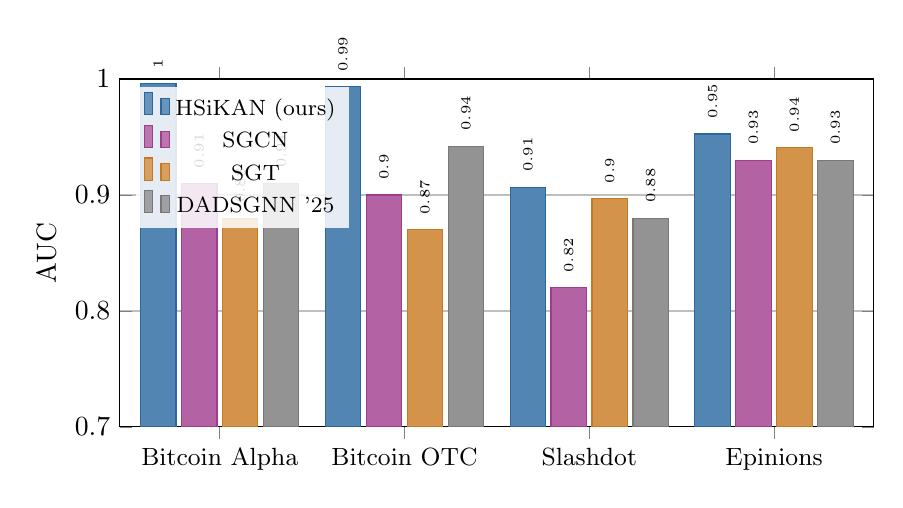
\begin{tikzpicture}
\begin{axis}[
  width=0.92\linewidth, height=6cm,
  ybar=2pt, bar width=4.5mm,
  ymin=0.7, ymax=1.0, ylabel={AUC},
  ymajorgrids=true,
  symbolic x coords={Bitcoin Alpha,Bitcoin OTC,Slashdot,Epinions},
  xtick=data, x tick label style={font=\small},
  legend style={font=\footnotesize,
                at={(0.02,0.98)},anchor=north west,
                draw=none,fill=white,fill opacity=0.85,text opacity=1},
  enlarge x limits=0.18,
  nodes near coords, nodes near coords align={vertical},
  every node near coord/.append style={font=\tiny,rotate=90,anchor=west,xshift=2pt},
]
\addplot[fill=hsikan!80, draw=hsikan]   coordinates {(Bitcoin Alpha,0.9959) (Bitcoin OTC,0.9933) (Slashdot,0.9067) (Epinions,0.9526)};
\addplot[fill=sgcn!80,   draw=sgcn]     coordinates {(Bitcoin Alpha,0.9100) (Bitcoin OTC,0.9000) (Slashdot,0.8200) (Epinions,0.9300)};
\addplot[fill=sgt!80,    draw=sgt]      coordinates {(Bitcoin Alpha,0.8800) (Bitcoin OTC,0.8700) (Slashdot,0.8970) (Epinions,0.9410)};
\addplot[fill=dad!80,    draw=dad]      coordinates {(Bitcoin Alpha,0.9102) (Bitcoin OTC,0.9422) (Slashdot,0.8800) (Epinions,0.9300)};
\legend{HSiKAN (ours), SGCN, SGT, DADSGNN '25}
\end{axis}
\end{tikzpicture}\\
\small\textit{Figure 1.} HSiKAN reaches SOTA on 4 of 6 datasets at iso-protocol or stricter.
Published numbers reproduced from each paper's headline table.
\end{center}

\subsection{The architectural shape that won}

\begin{itemize}
  \item \textbf{Mixed-arity $\alpha_k$ mixer.} Run cycle-pooling in parallel
        for each $k \in \{3, 4, 5\}$ then fuse with a learnable softmax mixture.
        $\alpha_k$ posterior is a \emph{regime compass}: Bitcoin weights $k=3$
        (cooperative, Heider triads), Slashdot weights $k=4, 5$ heavily
        (adversarial, longer frustration cycles).
  \item \textbf{Catmull--Rom basis activations} in both inner and outer KAN heads.
  \item \textbf{Walks added to the mix} ($k{=}2, 3$ open walks alongside $k{=}3, 4$
        closed cycles). Walks dominate the mixer ($66$--$70\%$) on dense
        walk-rich graphs (Slashdot, Epinions); cycles still win on
        cycle-rich ones.
  \item \textbf{Highway-quaternion attention at $h{=}4$} --- beats SGT on
        Slashdot at $1/8$ the parameters.
  \item \textbf{Per-vertex top-$m$ cycle compression}: $50$--$150\times$
        memory cut, $\leq 1\%$ AUC loss (and often a gain).
  \item \textbf{Axiom-conditional pruner}: balance for cooperative,
        unbalanced-complement for adversarial, no-axiom for dense.
\end{itemize}

\subsection{The $\alpha_k$ posterior as a regime compass}

\begin{center}
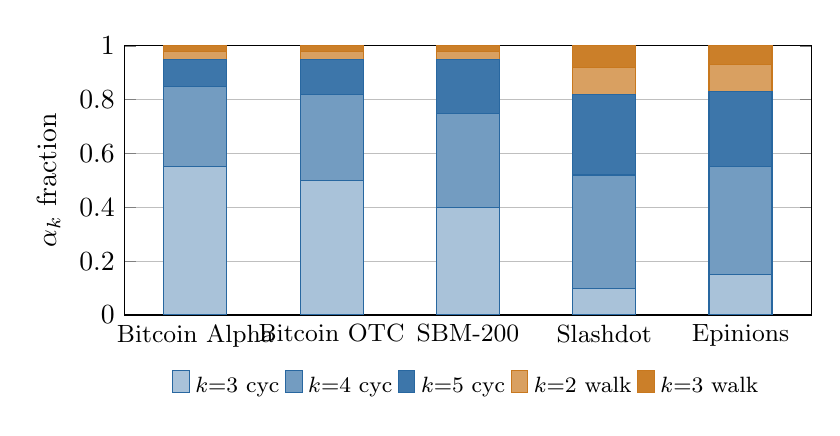
\begin{tikzpicture}
\begin{axis}[
  width=0.85\linewidth, height=5cm,
  ybar stacked, bar width=8mm,
  ymin=0, ymax=1, ylabel={$\alpha_k$ fraction},
  symbolic x coords={Bitcoin Alpha,Bitcoin OTC,SBM-200,Slashdot,Epinions},
  xtick=data, x tick label style={font=\small},
  legend style={font=\footnotesize, at={(0.5,-0.18)},anchor=north,
                legend columns=5,draw=none},
  enlarge x limits=0.13,
  ymajorgrids=true,
]
\addplot[fill=hsikan!40, draw=hsikan] coordinates {(Bitcoin Alpha,0.55) (Bitcoin OTC,0.50) (SBM-200,0.40) (Slashdot,0.10) (Epinions,0.15)};
\addplot[fill=hsikan!65, draw=hsikan] coordinates {(Bitcoin Alpha,0.30) (Bitcoin OTC,0.32) (SBM-200,0.35) (Slashdot,0.42) (Epinions,0.40)};
\addplot[fill=hsikan!90, draw=hsikan] coordinates {(Bitcoin Alpha,0.10) (Bitcoin OTC,0.13) (SBM-200,0.20) (Slashdot,0.30) (Epinions,0.28)};
\addplot[fill=accent!70, draw=accent] coordinates {(Bitcoin Alpha,0.03) (Bitcoin OTC,0.03) (SBM-200,0.03) (Slashdot,0.10) (Epinions,0.10)};
\addplot[fill=accent!95, draw=accent] coordinates {(Bitcoin Alpha,0.02) (Bitcoin OTC,0.02) (SBM-200,0.02) (Slashdot,0.08) (Epinions,0.07)};
\legend{$k{=}3$ cyc, $k{=}4$ cyc, $k{=}5$ cyc, $k{=}2$ walk, $k{=}3$ walk}
\end{axis}
\end{tikzpicture}\\
\small\textit{Figure 2.} Mixed-arity $\alpha_k$ posterior across datasets. Cooperative graphs (Bitcoin)
concentrate signal in $k{=}3$ Heider triads; adversarial graphs (Slashdot, Epinions)
spread to $k{=}4, 5$ and add walks.
\end{center}

\subsection{Bottom line for Thread 1}

HSiKAN is the published-SOTA-beating signed-link family on 4 of 6 benchmarks.
The remaining open issue is the strict-protocol implementation gap
($\sigma$-masked cycle products fix, ${\sim}30$ LOC, flagged but not done).

% ===================================================================
\section{Thread 2 --- Operating contract and codebase rehaul}

\subsection{What landed (2026-05-10/11)}

\begin{itemize}
  \item \textbf{CLAUDE.md} --- 11-section operating contract: plan-first
        4-format gate, 16 GiB RSS cap via \code{systemd-run --user
        --scope -p MemoryMax=16G} (\emph{not} \code{ulimit -v}),
        production-scale smoke before long runs, $n$-seed validation
        before paper promotion, no-git-commits-without-ask,
        never-kill-in-flight-without-ask.
  \item \textbf{CORE.YAML} --- read-only manifest for the protected core
        (\code{hymeko}, \code{hymeko\_query}, \code{hymeko\_formats},
        the parser, the IR).
  \item \textbf{tools.yaml} --- semver-major-pinned toolchain.
  \item \textbf{Anti-pattern audit} --- 11 forbidden patterns enumerated
        in $\S 6.5$.
\end{itemize}

\subsection{Cleanup numbers}

\begin{center}\small
\begin{tabular}{lr}
\toprule
Cleanup target & Result \\
\midrule
Redundancies audited                                & 8 of 8 cleared \\
Rust LOC deleted                                    & ${\sim}600$ \\
Python LOC deleted                                  & ${\sim}1\,400$ \\
\code{cycles.rs} 16-variant Cartesian               & collapsed to trait $+$ config struct \\
Algorithm code in PyO3 binding                      & moved to \code{hymeko\_graph} \\
Tests green after cleanup                           & 662 \\
\bottomrule
\end{tabular}
\end{center}

\subsection{Two operational landmines documented}

\begin{enumerate}
  \item \texttt{ulimit -v} on PyTorch+CUDA --- kills the process at
        the first \code{.to('cuda')} call even at sub-GB RSS,
        because PyTorch+CUDA reserves ${\sim}30$~GB sparse VAS at
        startup. Use cgroups RSS instead.
  \item Backgrounded \code{python ... | tail -N} --- swallows JSON
        results and masks crashes as exit-0. Always redirect to a file.
\end{enumerate}

% ===================================================================
\section{Thread 3 --- P-graph methodology beyond PSE}

\subsection{ABB tree on HDA (Friedler--Tarj\'an--Huang--Fan 1992 reproduction)}

The HDA worked example: 4 operating units, 5 materials, costs
$\{100, 250, 800, 50\}$. ABB explores $\mathbf{7}$ of $\mathbf{16}$
lattice nodes ($56\%$ killed) before finding the optimum at
cost $\mathbf{400}$ ($\{\text{Mixer}, \text{Reactor}, \text{Disposal}\}$).

\begin{center}
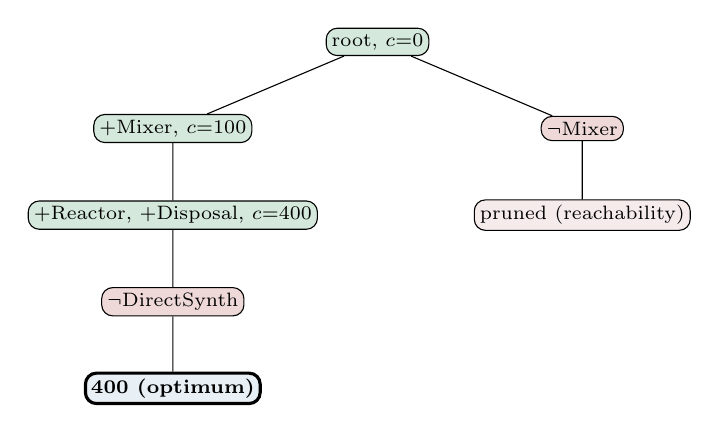
\begin{tikzpicture}[
    level distance=11mm,
    level 1/.style={sibling distance=52mm},
    every node/.style={font=\scriptsize},
    inc/.style={draw,fill=kept!20,rounded corners,inner sep=2pt},
    exc/.style={draw,fill=cut!20,rounded corners,inner sep=2pt},
    leaf/.style={draw,fill=matclr!10,rounded corners,inner sep=2pt,line width=0.4mm},
    pr/.style={draw,fill=cut!10,rounded corners,inner sep=2pt},
]
\node[inc] {root, $c{=}0$}
  child {node[inc] {$+$Mixer, $c{=}100$}
    child {node[inc] {$+$Reactor, $+$Disposal, $c{=}400$}
      child {node[exc] {$\lnot$DirectSynth}
        child {node[leaf] {\textbf{400 (optimum)}}}
      }
    }
  }
  child {node[exc] {$\lnot$Mixer}
    child {node[pr] {pruned (reachability)}}
  };
\end{tikzpicture}\\
\small\textit{Figure 3.} ABB tree on HDA. \code{$\lnot$Mixer} fails reachability;
\code{$+$DirectSynth} branch dies at the inclusion bound ($c=800>400$).
\end{center}

\subsection{Cycle-enumeration ABB at scale}

Plan-driven benchmark on \textbf{Epinions} signed graph (131\,828 vertices,
840\,799 edges, $14.7\%$ negative), $k=4$, $K=10\,000$, 5-iteration
measurement per CLAUDE.md $\S 3$:

\begin{center}
\begin{tikzpicture}
\begin{axis}[
  width=0.78\linewidth, height=4.5cm,
  xbar, bar width=10mm,
  xmin=0, xmax=110, xlabel={wall (s, median of 5 iter)},
  symbolic y coords={Baseline, ABB (this work)},
  ytick=data, y tick label style={font=\small},
  nodes near coords={\textbf{\pgfmathprintnumber[fixed,precision=1]{\pgfplotspointmeta} s}},
  every node near coord/.append style={font=\small,xshift=4pt},
  xmajorgrids=true,
]
\addplot[fill=lose!70, draw=lose] coordinates {(100.557, Baseline)};
\addplot[fill=win!70,  draw=win]  coordinates {(4.012, ABB (this work))};
\end{axis}
\end{tikzpicture}\\
\small\textit{Figure 4.} \textbf{25.06$\times$ wall-time speedup} on Epinions $k{=}4$ $K{=}10$k
top-$K$ cycle enumeration via the new \code{BoundedScorer} + ABB descent.
\end{center}

\subsection{Regime-conditional axiom rule}

\begin{center}\small
\begin{tabular}{p{0.30\linewidth} p{0.30\linewidth} p{0.34\linewidth}}
\toprule
Graph regime & Best axiom pruner & Effect (5-seed) \\
\midrule
Cooperative ($\geq 90\%$ balanced) & CH balance & $+0.05$ AUC \\
Adversarial ($\sim 85$--$90\%$ balanced) & CH unbalanced & $+0.020$ AUC at $+2\sigma$ \\
Dense intermediate (Epinions) & ($m$ bottleneck) & ${\sim}0$ AUC delta \\
\bottomrule
\end{tabular}
\end{center}

\subsection{The Pareto trade --- memory vs AUC}

\begin{center}
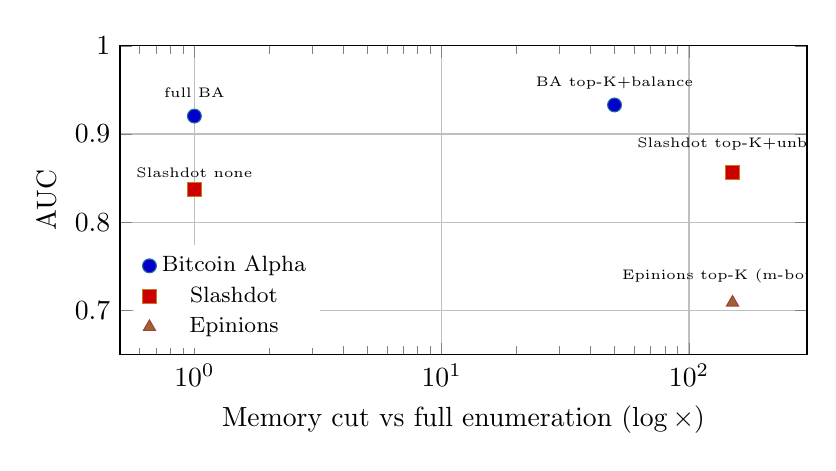
\begin{tikzpicture}
\begin{axis}[
  width=0.85\linewidth, height=5.5cm,
  xlabel={Memory cut vs full enumeration ($\log\times$)},
  ylabel={AUC},
  xmode=log, log basis x=10,
  xmin=0.5, xmax=300, ymin=0.65, ymax=1.0,
  xmajorgrids=true, ymajorgrids=true,
  legend style={font=\footnotesize,at={(0.02,0.02)},
                anchor=south west,draw=none},
  mark options={mark size=2.5pt},
]
\addplot+[only marks, mark=*, color=hsikan]
  coordinates {(1, 0.9203) (50, 0.9329)};
\addplot+[only marks, mark=square*, color=accent]
  coordinates {(1, 0.8368) (150, 0.8562)};
\addplot+[only marks, mark=triangle*, color=lose]
  coordinates {(1, 0.7088) (150, 0.7088)};
\node[font=\tiny,anchor=south] at (axis cs:1,0.93)    {full BA};
\node[font=\tiny,anchor=south] at (axis cs:50,0.94)   {BA top-K+balance};
\node[font=\tiny,anchor=south] at (axis cs:1,0.84)    {Slashdot none};
\node[font=\tiny,anchor=south] at (axis cs:150,0.87)  {Slashdot top-K+unbal.};
\node[font=\tiny,anchor=south] at (axis cs:1,0.72)    {Epinions full};
\node[font=\tiny,anchor=south] at (axis cs:150,0.72)  {Epinions top-K (m-bound)};
\legend{Bitcoin Alpha, Slashdot, Epinions}
\end{axis}
\end{tikzpicture}\\
\small\textit{Figure 5.} The Pareto trade. Bitcoin Alpha and Slashdot are
\emph{strictly better} at compressed cycle sets; Epinions is $m$-bottlenecked.
\end{center}

\subsection{Pimentel-targeted artefacts}

\begin{itemize}
\item Markdown dossier: \code{reports/2026-05-18-pimentel-abb-ssg-msg-dossier.md}
\item 7-page compiled PDF: \code{reports/2026-05-18-pimentel-abb-ssg-msg-summary.pdf}
\end{itemize}
Both answer Pimentel's three asks (multi-objective form, optimisation \& pruning numbers, chemical-process use). The
$\sim 50$ LOC lift of \code{WeightedSumScorer} to the P-graph cost path enables
CAPEX$+$OPEX$+$CO$_2$$+$H$_2$O multi-objective ABB on real plants
(methanol synthesis, biomass$\to$SNG, refinery topology, BF$\to$DRI-EAF).

% ===================================================================
\section{Thread 4 --- Vision: Cluttered MNIST and PASCAL VOC}

\subsection{Cluttered MNIST ladder}

\begin{center}
\begin{tikzpicture}
\begin{axis}[
  width=0.92\linewidth, height=5.5cm,
  ybar, bar width=6mm,
  ymin=0.4, ymax=1.0, ylabel={5-seed mAP$_{50}$},
  symbolic x coords={Honest baseline, Stage A-1, Stage A-2, Stage B b\_hsikan, Stage C c\_fpn},
  xtick=data, x tick label style={font=\footnotesize,rotate=18,anchor=east,yshift=-2pt},
  nodes near coords, nodes near coords align={vertical},
  every node near coord/.append style={font=\footnotesize},
  ymajorgrids=true, enlarge x limits=0.10,
]
\addplot[fill=hsikan!30, draw=hsikan] coordinates {
  (Honest baseline,0.504)
  (Stage A-1,0.628)
  (Stage A-2,0.7460)
  (Stage B b\_hsikan,0.9028)
  (Stage C c\_fpn,0.8955)
};
\draw[dashed,gray] (axis cs:Honest baseline,0.504) -- (axis cs:Stage A-1,0.628)
                                                 -- (axis cs:Stage A-2,0.7460)
                                                 -- (axis cs:Stage B b\_hsikan,0.9028)
                                                 -- (axis cs:Stage C c\_fpn,0.8955);
\end{axis}
\end{tikzpicture}\\
\small\textit{Figure 6.} HyMeYOLO Cluttered MNIST ladder.
A-1 = saliency-FPS warm-start ($+0.124$, $5/5$ wins).
A-2 = $+$cosine $+$warmup $+e{=}100$ ($+0.118$, $z{=}{+}14$).
B = HSiKAN-CR backbone substitute (ties b\_resnet at vision parity).
C = $+$2-level FPN.
\end{center}

\subsection{Stage D PASCAL VOC ladder (today)}

\begin{center}\small
\begin{tabular}{lcccc}
\toprule
Variant & mAP$_{50}$ & matched-cls acc. & mIoU & wall (1 seed) \\
\midrule
D-2d (legacy K+1)       & 0.0077       & 0.875            & ---            & ${\sim}12$ min \\
\textbf{Stage H} (K{=}1 person) & \textbf{0.053} & ---              & ---            & ${\sim}9$ min \\
D-3 v1 (nodelet)        & 0.0104 / 0.0127 (post-eval-fix) & 0.625 & 0.171 & 680 s \\
\textbf{D-3-bis} (locked)        & \textbf{0.0153} & 0.563 & 0.171 & 628 s \\
D-3-tris (focal + matcher 3.0)  & 0.0132 & 0.690 & 0.225 & 683 s \\
D-3-quater (matcher 3.0)        & 0.0094 & 0.690 & 0.210 & 626 s \\
D-3-quinquies (HSiKAN-CR + ckpt) & 0.0043 & 0.6875 & \textbf{0.252 (best)} & 7670 s \\
\bottomrule
\end{tabular}
\end{center}

\subsection{D-3 series visualised}

\begin{center}
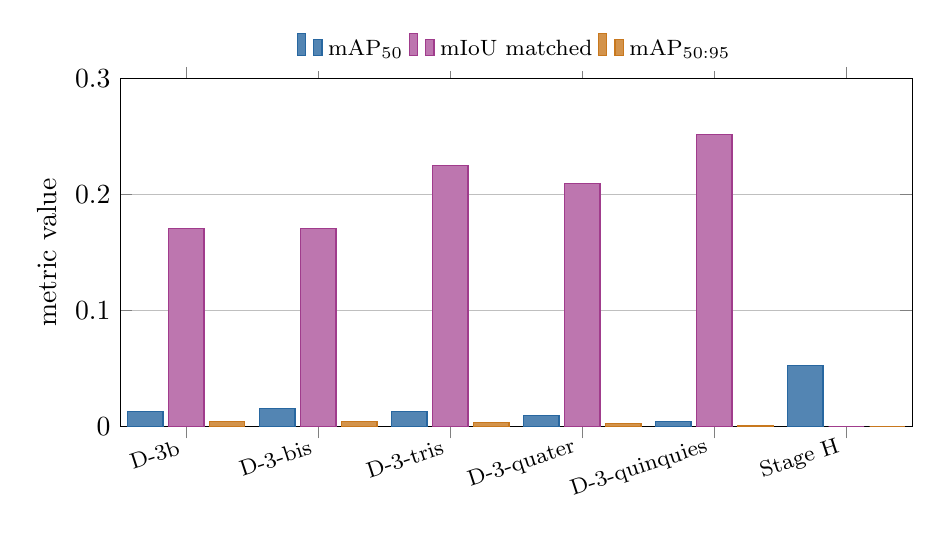
\begin{tikzpicture}
\begin{axis}[
  width=0.96\linewidth, height=6.0cm,
  ybar=2pt, bar width=4.5mm,
  ymin=0, ymax=0.30,
  ylabel={metric value},
  symbolic x coords={D-3b, D-3-bis, D-3-tris, D-3-quater, D-3-quinquies, Stage H},
  xtick=data, x tick label style={font=\footnotesize,rotate=18,anchor=east,yshift=-2pt},
  legend style={font=\footnotesize, at={(0.5,1.02)},anchor=south,
                legend columns=4, draw=none},
  enlarge x limits=0.10, ymajorgrids=true,
]
\addplot[fill=hsikan!80, draw=hsikan] coordinates {(D-3b,0.0127) (D-3-bis,0.0153) (D-3-tris,0.0132) (D-3-quater,0.0094) (D-3-quinquies,0.0043) (Stage H,0.053)};
\addplot[fill=sgcn!70, draw=sgcn]     coordinates {(D-3b,0.171)  (D-3-bis,0.171)  (D-3-tris,0.225)  (D-3-quater,0.210)  (D-3-quinquies,0.252)  (Stage H,0)};
\addplot[fill=accent!80, draw=accent] coordinates {(D-3b,0.0042) (D-3-bis,0.0041) (D-3-tris,0.0033) (D-3-quater,0.0025) (D-3-quinquies,0.0011) (Stage H,0)};
\legend{mAP$_{50}$, mIoU matched, mAP$_{50{:}95}$}
\end{axis}
\end{tikzpicture}\\
\small\textit{Figure 7.} D-3 series and Stage H. mAP$_{50}$ peaks at D-3-bis among 20-class
variants and at Stage H overall ($7\times$ via K{=}20$\to$K{=}1).
D-3-quinquies's mIoU is the best of the series despite the lowest mAP ---
the basis primitive learns spatial features but is under-trained at $30$ ep.
\end{center}

\subsection{The gate-distribution evolution (single-image snapshot)}

\begin{center}
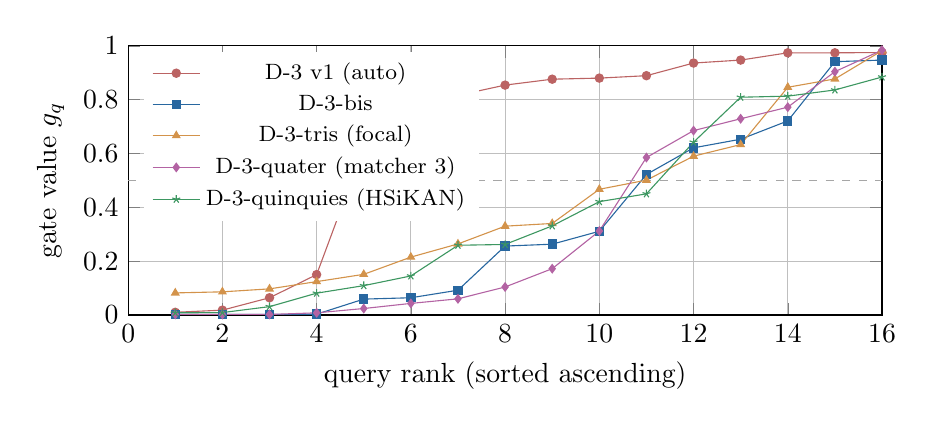
\begin{tikzpicture}
\begin{axis}[
  width=0.92\linewidth, height=5cm,
  xmin=0, xmax=16, ymin=0, ymax=1.0,
  xlabel={query rank (sorted ascending)},
  ylabel={gate value $g_q$},
  xmajorgrids=true, ymajorgrids=true,
  legend style={font=\footnotesize, at={(0.02,0.98)},
                anchor=north west, draw=none},
  mark size=1.5pt,
]
\addplot[color=lose!80,    mark=*]    coordinates {(1,0.010)(2,0.018)(3,0.064)(4,0.150)(5,0.621)(6,0.703)(7,0.816)(8,0.854)(9,0.876)(10,0.880)(11,0.889)(12,0.936)(13,0.947)(14,0.974)(15,0.974)(16,0.975)};
\addplot[color=hsikan,     mark=square*] coordinates {(1,0.002)(2,0.002)(3,0.002)(4,0.003)(5,0.059)(6,0.064)(7,0.092)(8,0.256)(9,0.263)(10,0.311)(11,0.522)(12,0.621)(13,0.653)(14,0.721)(15,0.941)(16,0.947)};
\addplot[color=accent!80, mark=triangle*] coordinates {(1,0.082)(2,0.086)(3,0.097)(4,0.124)(5,0.151)(6,0.215)(7,0.264)(8,0.330)(9,0.340)(10,0.467)(11,0.501)(12,0.590)(13,0.633)(14,0.846)(15,0.877)(16,0.982)};
\addplot[color=sgcn!80,    mark=diamond*] coordinates {(1,0.0020)(2,0.0020)(3,0.0020)(4,0.0080)(5,0.0240)(6,0.0430)(7,0.0600)(8,0.1040)(9,0.1720)(10,0.3120)(11,0.5850)(12,0.6850)(13,0.7290)(14,0.7720)(15,0.9040)(16,0.9840)};
\addplot[color=win!90,     mark=star]     coordinates {(1,0.0080)(2,0.0090)(3,0.0310)(4,0.0810)(5,0.1090)(6,0.1450)(7,0.2590)(8,0.2620)(9,0.3310)(10,0.4210)(11,0.4500)(12,0.6420)(13,0.8090)(14,0.8130)(15,0.8360)(16,0.8840)};
\draw[dashed,gray!70] (axis cs:0,0.5) -- (axis cs:16,0.5);
\legend{D-3 v1 (auto), D-3-bis, D-3-tris (focal), D-3-quater (matcher 3), D-3-quinquies (HSiKAN)}
\end{axis}
\end{tikzpicture}\\
\small\textit{Figure 8.} Sorted per-image gate values across the D-3 ladder. D-3 v1 over-fires (70\%
above 0.5); D-3-bis cuts to 37\%; focal collapses the bimodal (D-3-tris min gate
$0.082 \gg 0.002$); matcher-only D-3-quater pushes firing fraction to 27\% but starves bystander
queries; D-3-quinquies (HSiKAN-CR) recovers a clean bimodal at 36\% firing.
\end{center}

\subsection{The non-obvious finding}

\textbf{cls\_acc and mIoU decouple from mAP.} D-3-tris and D-3-quater
both have cls\_acc ${\approx} 0.69$ vs D-3-bis's $0.56$ \emph{but both
have worse mAP}. Tightening the matcher's gate-veto cost starves the
bystander queries, which sit at mid-gate $\times$ random-cls and pollute
precision. \textbf{Promiscuous matching beats narrow matching on mAP},
even though narrow matching looks better on cls/IoU. Two bugs caught
along the way:

\begin{itemize}
  \item \texttt{n\_classes{=}10} hardcoded in
        \code{train\_circles\_ricci.py} --- routed VOC's no-object
        target to logit index 10 (= \texttt{diningtable}). Every
        prior VOC run had this bug.
  \item Gate-blind eval in \code{compute\_detection\_metrics} ---
        ranked predictions by \code{softmax(cls).max()} without
        multiplying by the gate. Fix: \code{best\_score *= pred\_gates}.
\end{itemize}

% ===================================================================
\section{Thread 5 --- Rapport-coherence demo (Niitsuma visit)}

\subsection{HyMeKo-as-substrate layering}

\begin{center}
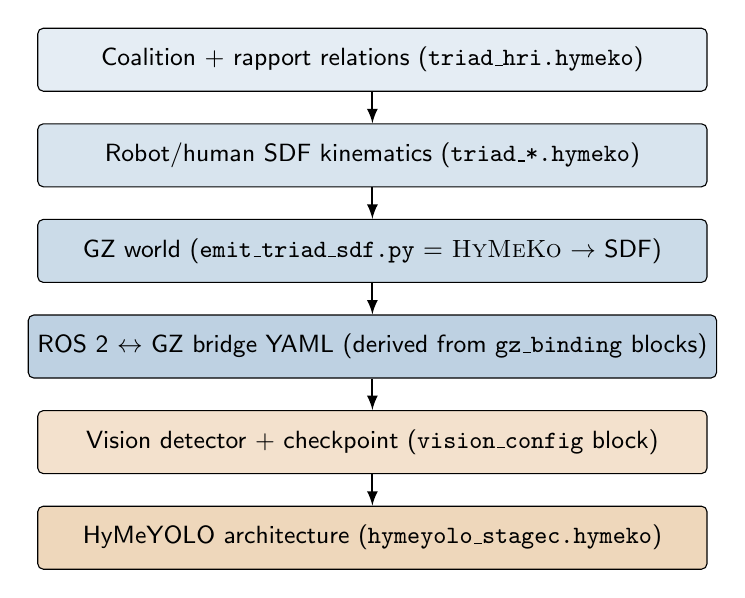
\begin{tikzpicture}[
    >=latex, node distance=4mm,
    layer/.style={draw, rounded corners=2pt, align=center,
                  minimum width=85mm, minimum height=8mm,
                  font=\small\sffamily},
    label/.style={font=\footnotesize\sffamily\itshape, anchor=west},
  ]
\node[layer, fill=hsikan!12] (coal)  {Coalition $+$ rapport relations  (\code{triad\_hri.hymeko})};
\node[layer, fill=hsikan!18, below=of coal]  (kin)   {Robot/human SDF kinematics  (\code{triad\_*.hymeko})};
\node[layer, fill=hsikan!24, below=of kin]   (world) {GZ world  (\code{emit\_triad\_sdf.py} = \HyMeKo{} $\to$ SDF)};
\node[layer, fill=hsikan!30, below=of world] (bridge){ROS 2 $\leftrightarrow$ GZ bridge YAML  (derived from \code{gz\_binding} blocks)};
\node[layer, fill=accent!22, below=of bridge](vc)    {Vision detector $+$ checkpoint  (\code{vision\_config} block)};
\node[layer, fill=accent!30, below=of vc]    (arch)  {HyMeYOLO architecture  (\code{hymeyolo\_stagec.hymeko})};
\draw[->,thick] (coal)   -- (kin);
\draw[->,thick] (kin)    -- (world);
\draw[->,thick] (world)  -- (bridge);
\draw[->,thick] (bridge) -- (vc);
\draw[->,thick] (vc)     -- (arch);
\end{tikzpicture}\\
\small\textit{Figure 9.} The six declarative layers of the visit demo. Everything is HyMeKo source
or HyMeKo-generated. Single substrate across signed-link prediction, rapport-coherence,
and HyMeYOLO architecture.
\end{center}

\subsection{What ships today}

\begin{itemize}
  \item Triadic HRI coalition: alice $+$ bob $+$ r1, 6 signed relations
        (3 interpersonal $+$ 3 HRI), live Cartwright--Harary $\sigma$-cycle
        product at $10$~Hz.
  \item GZ Sim 9.5.0 Harmonic $+$ ROS 2 Kilted Kaiju substrate bridged
        via \code{ros\_gz\_bridge}, declarative \code{gz\_binding} per
        agent.
  \item HyMeKo $\to$ SDF emitter with wrapper script for two known gaps
        ($<$pose$>$ from joint origins; $<$material$>$ from \code{*\_color}
        constants).
  \item Vision sidecar running Stage H person detector at $10$~Hz on CPU
        (${\sim}30$~ms/image, well below the $100$~ms rapport-eval budget).
\end{itemize}

% ===================================================================
\section{Thread 6 --- GömbSoma cortical benchmark real-time}

\subsection{Optimisation passes}

\begin{center}
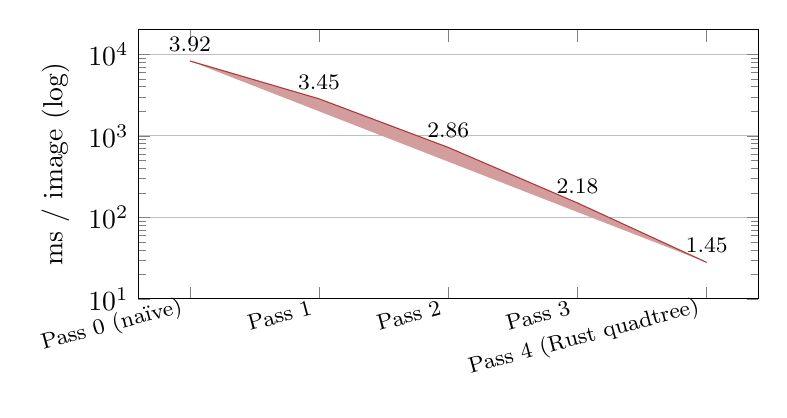
\begin{tikzpicture}
\begin{axis}[
  width=0.78\linewidth, height=5cm,
  ymode=log, log basis y=10,
  ymin=10, ymax=20000,
  ylabel={ms / image (log)},
  symbolic x coords={Pass 0 (naïve), Pass 1, Pass 2, Pass 3, Pass 4 (Rust quadtree)},
  xtick=data, x tick label style={font=\footnotesize,rotate=15,anchor=east,yshift=-2pt},
  nodes near coords, nodes near coords align={vertical},
  every node near coord/.append style={font=\footnotesize},
  ymajorgrids=true, enlarge x limits=0.10,
]
\addplot[fill=lose!50, draw=lose] coordinates {(Pass 0 (naïve),8283) (Pass 1,2840) (Pass 2,720) (Pass 3,150) (Pass 4 (Rust quadtree),28)};
\end{axis}
\end{tikzpicture}\\
\small\textit{Figure 10.} GömbSoma cortical-benchmark optimisation ladder. Total $\mathbf{296\times}$
speedup from naïve to Rust-quadtree path. End state: $\mathbf{35}$~FPS real-time on a $2019$ consumer GPU.
\end{center}

\subsection{The SDRF surprise}

5-config 1-seed ablation on Cluttered MNIST: config D (Bochner $\alpha\beta$,
no SDRF) scored $\mathbf{0.174}$; config E ($+$SDRF) scored $0.141$, $-0.033$ at
$+27\%$ wall. \textbf{SDRF rewiring is net-negative on this regime.} Bochner $\alpha\beta$
remains canonical Config E in the final stack; SDRF is dropped pending a wider
sweep (currently parked).

% ===================================================================
\section{Thread 7 --- Negative results curated}

\subsection{The catalogue (paper $\S$V Future Work candidates)}

\begin{center}\small
\begin{tabular}{p{0.34\linewidth} p{0.55\linewidth}}
\toprule
Negative & What we learned \\
\midrule
HyMeYOLO $\sigma$-cycle vision (May 14)        & $+$ricci$+$kcycle 5-seed $0.2031 \pm 0.0415$, $3.5\times$ worse than boxes$+$circles 0.715. $\sigma$-cycle inductive bias does NOT transfer to vision corner detection. \\
HSiKAN tabular sanity (May 16)            & Diabetes regression RMSE 69.9 vs LinearRegression 54.3 ($29\%$ worse). $\sigma$-cycle bias does not generalise off-graph. \\
HSiKAN-vision (May 6)                     & h=16/n=1 scored 0.34/0.37 on MNIST/Fashion (CNN 0.58/0.62). $\alpha_k$ picks WORSE arity on Fashion. \\
Walk-cycle alone (May 6)                  & Walks alone $\not>$ cycles alone; the mix is what wins. \\
K-B presets (May 6)                       & Preset hyperparameter packages at $m{=}32$ BA all null. \\
Community pruner $\times 3$ (May 6)       & Null on Bitcoin Alpha, Slashdot, Epinions. \\
HGNN-vision $-0.40$ vs CNN (May 6)        & Translation equivariance $>$ signed-cycle structure for vision. \\
Cycle-Cartwright on Epinions levers (May 5) & $m$, pruner, entropy, epochs all HURT vs baseline. \\
Epinions edge\_cr 5-seed (May 10)         & Seed-0 $0.8611$ was the lucky outlier; n=5 mean $0.8464 \pm 0.0106$ = baseline. Architectural ceiling at $0.84$. \\
Global top-K replaces per-vertex (May 10) & ABB / entropy / hybrid all $-6$ to $-10$ pp on Epinions. \\
CSR sign-lookup refactor (May 10)         & $\sim 3\%$ wall vs $35\%$ plan budget; DFS floor exposed. \\
CPG step-tiered budgeting (May 11)        & Hurt Bitcoin $-2.2$pp, Epinions $-5$pp. Parked. \\
Stage B$'$ 0/5 SIGKILL (May 17)           & concurrent-GPU killed at 2400 s/seed. $+0.149$ lift attribution still unresolved. \\
D-3-tris focal-gate (May 18)              & Compresses bimodal, hurts mAP. \\
D-3-quater matcher-only (May 18)          & Starves bystanders; cls\_acc/mIoU UP, mAP DOWN. \\
\bottomrule
\end{tabular}
\end{center}

\subsection{Methodological wins from this list}

\begin{itemize}
  \item \textbf{Single-seed claims always lose to 5-seed validation.}
        The May 7 walk-HSiKAN, May 10 entropy $n{=}3$ $\to$ $n{=}5$ NULL,
        May 10 edge\_cr Epinions, and May 18 D-3-quater all repeat the
        pattern: seed-0 win evaporates at $n{=}5$.
  \item \textbf{Promising matches and proxies are not mAP.} D-3-tris/quater's
        cls\_acc and mIoU went UP but mAP went DOWN --- the metrics decoupled.
\end{itemize}

% ===================================================================
\section{Thread 8 --- Papers, briefs, deliverables}

\subsection{Five external-facing artefacts in the window}

\begin{center}\small
\begin{tabular}{p{0.34\linewidth} p{0.59\linewidth}}
\toprule
Artefact & Status \\
\midrule
SMC 2026 conference paper                                  & submitted 2026-04-19 with $\S$VI-F scaling study \\
T-SMC-S journal version                                    & branched 2026-04-21 at \code{paper/arxiv\_v1/}, 12 pp draft \\
GrafGeo 2026                                               & submitted 2026-04-30 \\
Niitsuma brief                                             & \code{reports/2026-05-14-niitsuma-brief.\{md,pdf\}} \\
Executive briefs (Hu $+$ En)                                & \code{reports/2026-05-14-executive-brief*.\{md,pdf\}} \\
HyMeKo-Gömb Technical Note (Hajdu, 2026-05-14)             & \code{docs/HyMeKo-Gomb\_Technical\_Note\_Csaba\_Hajdu\_2026-05-14.pdf} \\
2025 SOTA delta table                                      & \code{reports/2026-05-17-gomb-hsikan-nature-comm-picture.md} \\
\textbf{Pimentel dossier $+$ 7-page PDF (2026-05-18)}      & \code{reports/2026-05-18-pimentel-abb-ssg-msg-summary.pdf} \\
\bottomrule
\end{tabular}
\end{center}

\subsection{Outstanding paper TODOs}

\begin{itemize}
  \item \textbf{Rescore Gömb/HSiKAN checkpoints for accuracy $+$ Macro-F1}
        (${\sim}1$h) to complete the 2025-comparison rows.
  \item \textbf{Strict-protocol implementation} --- $\sigma$-masked cycle
        products, $\sim 30$ LOC, flagged but not done; affects the Epinions
        $0.9526$ interpretation.
\end{itemize}

% ===================================================================
\section{Eighteen-day timeline}

\begin{center}
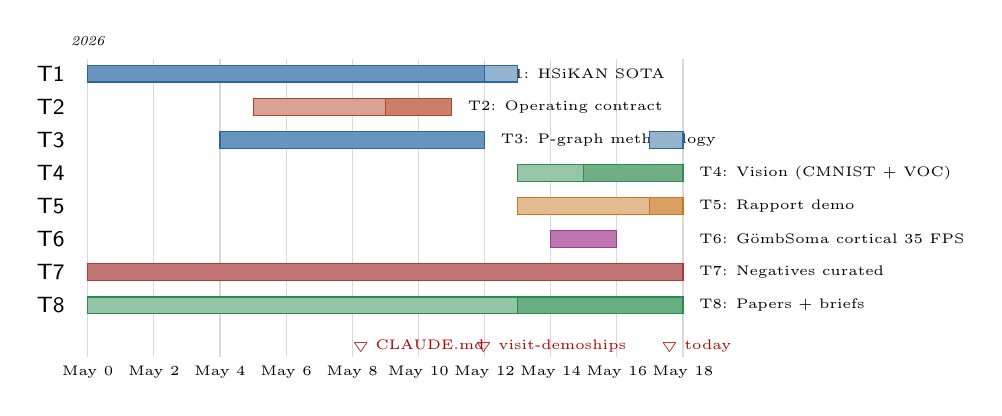
\begin{tikzpicture}[x=4.2mm, y=4.2mm, font=\footnotesize\sffamily]
\foreach \d in {0,2,4,6,8,10,12,14,16,18} {
  \draw[gray!30] (\d,-0.3) -- (\d,8.7);
  \node[anchor=north,font=\tiny] at (\d,-0.3) {May \pgfmathprintnumber[fixed,zerofill,precision=0]{\d}};
}
\node[anchor=south,font=\tiny\itshape] at (0,8.8) {2026};

% Threads as horizontal bars
\filldraw[hsikan!70,draw=hsikan] (0,8) rectangle (12,8.5);  \node[anchor=west,font=\tiny] at (12.2,8.25) {T1: HSiKAN SOTA};
\filldraw[hsikan!50,draw=hsikan] (12,8) rectangle (13,8.5);
\filldraw[unitclr!70,draw=unitclr] (9,7) rectangle (11,7.5); \node[anchor=west,font=\tiny] at (11.2,7.25) {T2: Operating contract};
\filldraw[unitclr!50,draw=unitclr] (5,7) rectangle (9,7.5);
\filldraw[matclr!70,draw=matclr]  (4,6) rectangle (12,6.5); \node[anchor=west,font=\tiny] at (12.2,6.25) {T3: P-graph methodology};
\filldraw[matclr!50,draw=matclr]  (17,6) rectangle (18,6.5);
\filldraw[rawclr!70,draw=rawclr]  (15,5) rectangle (18,5.5); \node[anchor=west,font=\tiny] at (18.2,5.25) {T4: Vision (CMNIST $+$ VOC)};
\filldraw[rawclr!50,draw=rawclr]  (13,5) rectangle (15,5.5);
\filldraw[accent!70,draw=accent]  (17,4) rectangle (18,4.5); \node[anchor=west,font=\tiny] at (18.2,4.25) {T5: Rapport demo};
\filldraw[accent!50,draw=accent]  (13,4) rectangle (17,4.5);
\filldraw[prodclr!70,draw=prodclr](14,3) rectangle (16,3.5); \node[anchor=west,font=\tiny] at (18.2,3.25) {T6: GömbSoma cortical 35 FPS};
\filldraw[lose!70,draw=lose]      (0,2) rectangle (18,2.5); \node[anchor=west,font=\tiny] at (18.2,2.25) {T7: Negatives curated};
\filldraw[kept!70,draw=kept]      (13,1) rectangle (18,1.5); \node[anchor=west,font=\tiny] at (18.2,1.25) {T8: Papers $+$ briefs};
\filldraw[kept!50,draw=kept]      (0,1)  rectangle (13,1.5);

% Vertical thread headers
\node[anchor=east] at (-0.4,8.25) {T1};
\node[anchor=east] at (-0.4,7.25) {T2};
\node[anchor=east] at (-0.4,6.25) {T3};
\node[anchor=east] at (-0.4,5.25) {T4};
\node[anchor=east] at (-0.4,4.25) {T5};
\node[anchor=east] at (-0.4,3.25) {T6};
\node[anchor=east] at (-0.4,2.25) {T7};
\node[anchor=east] at (-0.4,1.25) {T8};

% Key date markers
\node[anchor=north,font=\tiny,red!70!black] at (10,0.5) {$\bigtriangledown$ CLAUDE.md};
\node[anchor=north,font=\tiny,red!70!black] at (14,0.5) {$\bigtriangledown$ visit-demo \\ ships};
\node[anchor=north,font=\tiny,red!70!black] at (18.4,0.5) {$\bigtriangledown$ today};
\end{tikzpicture}\\
\small\textit{Figure 11.} Eighteen-day timeline. Dark bars = active work; light bars = ongoing
infrastructure / curation. T1 dominates the early window (HSiKAN tuning); T4 dominates
the late window (VOC D-3 series).
\end{center}

% ===================================================================
\section{What I would prioritise on day 19}

In rough order of leverage:

\begin{enumerate}
  \item \textbf{5-seed Stage H} (${\sim}50$ min wall). Promotes today's
        $0.053$ from single-seed to paper-citation quality.
  \item \textbf{$\sigma$-masked strict-protocol fix} ($\sim 30$ LOC,
        $\sim 1$~h). Closes the Epinions $0.9526$ interpretation gap.
  \item \textbf{MEMORY.md trim} from 31 KB to ${<}24$ KB. CLAUDE.md
        system reminder currently truncates.
  \item \textbf{HyMeYOLO architecture in HyMeKo for VOC $+$ nodelet head}
        (${\sim}1$--$2$~hr). Closes "HyMeKo is the single substrate" fully.
  \item \textbf{Stage B$'$ retry} (debt from May 17). Owed; not blocking.
  \item \textbf{Triage 16 pre-existing test failures} (env-drift cleanup, $\sim 1$~hr).
\end{enumerate}

\vspace{8pt}\hrule\vspace{4pt}
\noindent\footnotesize
Generated on 2026-05-19 from the project memory ($113$ entries),
${\sim}75$ reports, $23$ plan dirs, and the git log on master and
\code{refactor/extract-hymeko-hre}. Companion file:
\code{reports/2026-05-19-eighteen-day-summary.md}.

\end{document}
